\chapter{Planning et évolutions}

% Section Évolution du planning
%  - présentation des Gantt
%  - discussion sur leur évolution et les raisons

%\begin{figure}[h]
%  \caption{\label{ganttX} }
%  \includegraphics[width=15cm]{images/ganttXX}
%\end{figure}

\section{Planning initial}

Le planning initial illustré par la figure \ref{gantt1}
prévoyait que la majorité du projet serait terminée avant
mi-décembre, ne laissant pour la fin d'année que la correction
de détails et la rédaction du mémoire final.

\begin{figure}[h]
  \caption{\label{gantt1} Planning prévisionnel initial}
  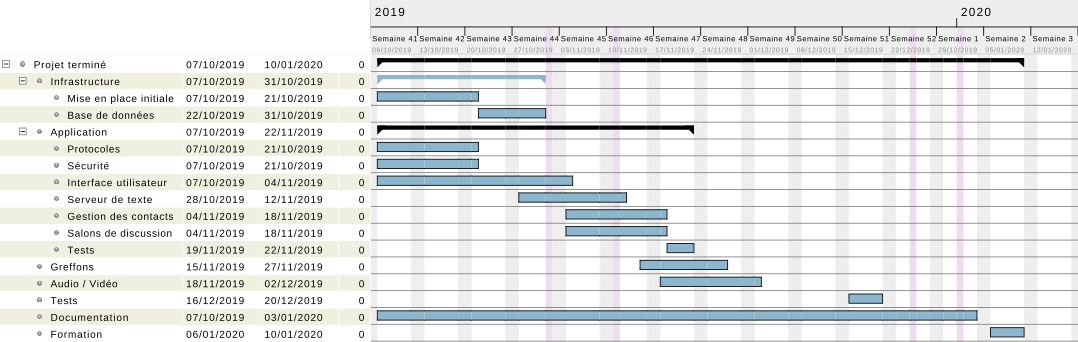
\includegraphics[width=15cm]{images/gantt01}
\end{figure}

Les tâches du planning initial étaient très peu subdivisées,
ce qui n'a pas facilité l'estimation de la charge de travail
requise pour les accomplir et est sans doute l'un des facteurs
ayant conduit à certains retards.

Nos prévision étaient que chaque tâche majeur prendrait deux
semaines à réaliser. Si cette estimation était probablement
vrai pour certaines tâches de conception, un découpage plus
fin comme celui du dernier Gantt illustré par la figure
\ref{gantt5} nous aurait permis de voir plus facilement le
travail impliqué par chaque tâche.

De plus, notre inexpérience a conduit à des imprécisions dans
nos documents initiaux, et des flous en terme de choix
techniques. Les enjeux en la matière ayant été mal compris,
nous avons du faire valider plusieurs choix par nos clients,
ce qui nous a ralenti davantage, car plusieurs échanges de
requête réponse entre humains prennent rapidement une à deux
semaines.

\subsection{Planning final}

Au fil des retards successifs notre organisation a pris la
forme illustrée par la figure \ref{gantt5}, présentant une
liste de tâches plus détaillée, avec des tâches divisées en
tâches plus petites et plus courtes, aboutissant à des tâches
effectives plus longues que ce que nous avions prévu à
l'origine.

\begin{figure}[h]
  \caption{\label{gantt5} Planning prévisionnel final}
  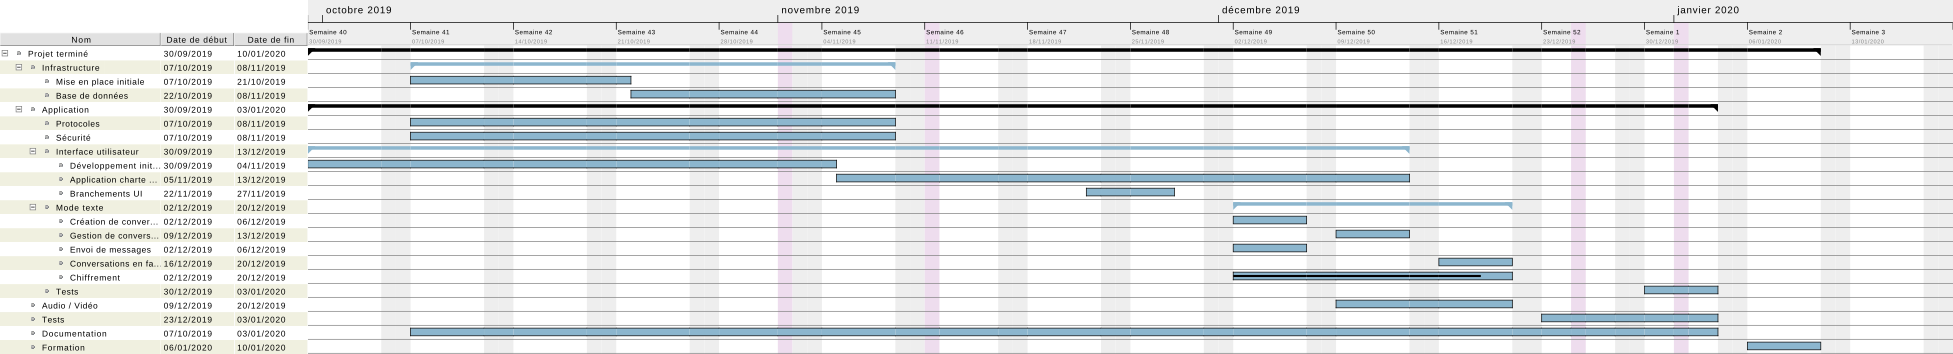
\includegraphics[width=15cm]{images/gantt05}
\end{figure}

Finalement le projet a avancé beaucoup moins rapidement que
ce que nous prévoyions, et ce que Gabriel avait prévu dès le
départ arrivé sur la fin, la période des fêtes de fin d'année
et les vacances associées ont été une période globalement très
peu productive.

\subsection{Outil utilisé}

L'outil \textit{Gantt Project} utilisé pour réaliser ces
diagrammes possède des capacités peu utilisées par le chef
de projet : les graphes de dépendances notamment, qui auraient
permis une représentation plus visuelle du travail à faire,
et du travail déjà fait. La gestion des ressources également,
une fonctionnalité mal documentée et mal compris du logiciel
qui auraient permis de facilité le calcul des coûts lors des
phases initiales du projet.
